\documentclass{article}
\usepackage{vmlmacros}
\usepackage{simplebnf}
\usepackage{tikz}
\usepackage{float}
\floatstyle{boxed} 
\restylefloat{figure}

\begin{document}

    \section{Will boolean expressions work?}

    We have discussed the necessity to limit 'intervening' computation in an
    equation, a pattern, or a decision tree let-node. Equations often 
    use intermediate expressions for their boolean result to decide whether 
    to continue computation, like: 

    \[\lambda y.\; \exists x.\; x = 2; \bf{x $\leq$ y}; x \]

    (The intermediate expression here is shown in bold for emphasis).
    
    The boolean nature of these expressions suggests that we might limit such
    intervening expressions to be purely boolean-based. We do not have a type
    system to do this, so we would have to use syntactic restriction:
    computation involving only values, names, boolean operators (\tt{\&\& || !
    $\geq$ $\leq$ $\lt$ $\gt$ etc.}) We could even add $\lambda$, where 
    the body of a lambda is of such a restricted form. It might look like this:

    \newcommand{\eb}{\ensuremath{e_{b}}}

    \begin{center}
        \begin{bnf}
            $\eb$ : boolean expressions ::= \tt{true}
            | \tt{false}
            | $x, y, z$ : names 
            | $e_{b_{1}}\; \tt{boolbinop}\; e_{b_{2}}$ 
            | $! \eb$ 
            ;;
            $\tt{boolbinop}$ : binary boolean operators ::= \tt{\&\&}
            | $\vert\vert$ : Sorry, I couldn't get these 
            | $\geq$       : bars into teletype
            | $\leq$       : and wrestling with it
            | \tt{>}       : didn't seem important rn.
            | \tt{<}
            | \tt{!=} 
            ;;
        \end{bnf}
    \end{center}
    

    This may seem a beneficial pattern, given its reusability in 
    decision tree nodes: 
    \begin{center}
        \begin{bnf}
            $\Dalpha$ : Decision trees ::= \dots 
            | $\tt{let}\; x\; \tt{=}\; \eb\; \tt{in}\; \Dalpha$ : let-bind a name
            | | $\tt{if}\; x\; \tt{then}\; \Dalpha\; \tt{else}\; \Dalpha$ : condition with two children 
            
        \end{bnf}
    \end{center}

    However, as we will see in the following section, there are large issues
    with this when we a) move to Verse and b) attempt to build decision trees
    from pattern guards. 

\section{The troubles}

There are several problems to this approach: 

\begin{enumerate}
    \item Verse expressions don't evaluate to true and false; they evaluate to a
          sequence of values, where the empty sequence \fail\; is used as
          falsehood. So, one would need a different representation of
          intermediate Verse expressions, somewhat defeating the purpose 
          of a universal boolean-expression form. 
    \item When we need to compile a pattern guard, like so: \\
        \tt{case l of (x::xs) ; (SOME y <- lookup rho x) ; y > 3 => y \\
            \it{\dots other patterns here \dots}} \\
        with \tt{lookup: 'a env -> name -> 'a option} \\
        \it{(please excuse the insane mix of syntax and typed/untyped bases; 
        this is to express just the idea)} \\
        we find the need to perform a function call, namely 
        \tt{lookup}, mid-tree traversal. 

        Our tree looks a bit like this: 


\bigskip
\begin{figure}[H]
    \centering
    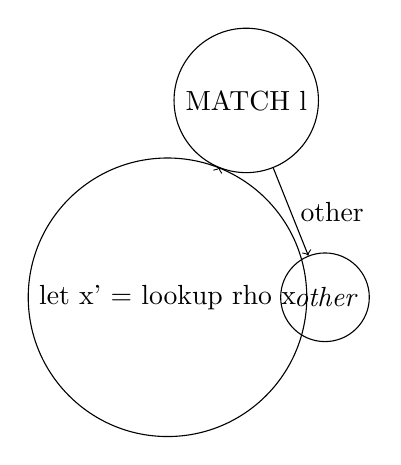
\begin{tikzpicture}
        \node[circle, draw] (1) at (5,10) {MATCH l};
        \node[circle, draw] (2) at (4,7.5) {let x' = lookup rho x};
        \node[circle, draw] (3) at (6,7.5) {\it{other}};
        % \node[circle, draw] (4) at (5.5,0) {SML};


        \draw[->] (1) to node[left] {\cons} (2);
        \draw[->] (1) to node[right] {other} (3);
        % \draw[->] (3) to (4);
        % \draw[->] (1) to[bend right] (3);
    \end{tikzpicture}
    \caption{Flow of language translation.}
    \label{fig:graph}
\end{figure}
\end{enumerate}

\end{document}